\section{Effects on Selection}
I begin this section by presenting descriptive evidence on the nature of selection into immigration from China to Canada at the start of the Head Tax period in the 1880's, and how selection evolved as the Head Tax grew. I then introduce a differences-in-differences empirical strategy to test for the effect of the Head Tax on selection, and present the results.

\subsection{Descriptive Evidence}
To identify whether immigrants are selected negatively or positively on skill relative to the origin country population requires representative skill data on two populations: the immigrant population and the origin country population. For the former I use the Chinese Register. While the Register covers the universe of legal Chinese immigrants to Canada between 1886 and 1923, it contains limited information and no direct measures of skill in the form of education or literacy. To measure selection in this data I use height, a common metric of human capital in the economic history literature, particularly in the context of historical selection into migration \citep{humphriesleunig2009,stolzbaten2012,kosackward2014,EscamillaGuerreroLopezAlonso2023}. 
Unlike other measures of selection such as wages or education, after a certain age height is largely independent of any further human capital investment and therefore cannot be affected by the decision to migrate. Additionally, since height was measured by immigration officials at the time of registration, it is likely more accurately and consistently measured than other self-reported variables in the Chinese Register, such as occupation.

Obtaining any data on the native Chinese population in the 19th century poses a significant hurdle. The biggest advantage of using height as a metric of selection is that it has been used in other settings to measure the human capital of the Chinese population in the 19th and early 20th centuries, and while I do not have raw data on the height in China during this time period, I can use estimates from previous work to characterize the height of the origin population \citep{olds2003, morgan2004, carson2006, batenhira2008, morgan2009, batenetal2010}.\footnote{\citet{olds2003} uses data from 1921-1931 during the Japanese occupation of Taiwan; \citet{morgan2004} uses records of Chinese government employees in the 1930s and 1940s; 
\citet{carson2006} uses data on Chinese immigrants who were imprisoned in the Western U.S. during the 19th century; 
\citet{batenhira2008} use data on contract migrants from China to Suriname and Indonesia collected in the 1880s; 
\citet{morgan2009} uses data on Chinese immigrants to Australia who were imprisoned in Melbourne between 1853 and 1927;
\citet{batenetal2010} compile several of the above data and add a small dataset of Chinese migrants to the U.S. collected between 1907 and 1948. All data focus on men of Chinese ethnicity from Guangdong (excluding \citet{olds2003}, which looks at Taiwan), the province from which over 96\% of Chinese immigrants in the Register originated.}

\vspace{2mm}
\noindent \textbf{Initial Selection} \par 
The average height of Chinese men who immigrated to Canada from 1886-1900 between the ages of 23 and 50 was 163.4cm.\footnote{Following the literature, I exclude men below the age of 23 who may not have finished growing at the time of migration, and men above the age of 50 who may have begun to shrink in height \citep{batenetal2010}. Since a large fraction of Chinese immigrants were young men, this excludes roughly 40\% of the sample.} While potentially biased by outmigration and selection into registration, the average height of Chinese men who immigrated to Canada before 1886 at ages 23-50 was similar if slightly lower, at 162.8cm. How do these estimates compare to the average height of Chinese men at the time?

The first set of benchmark figures that I use is from \citet{olds2003}, who uses data on Taiwanese men collected between 1920 and 1930 under Japanese occupation. Unlike data on migrants, these data cover the entire population, and so are not biased by selection into migration, and are likely representative of height in Southern China due Taiwan's geographic proximity and socioeconomic similarity to Southern China during the late 19th century.\footnote{Taiwan was under Qing rule until 1895, when it was ceded to Japan, so Taiwanese men born before 1870 would have grown to their full height under similar conditions to Southern Chinese men born at the same time.} 
\citet{olds2003} estimates that after adjusting for age-related shrinkage and death patterns, the average height for an adult Taiwanese man born between 1860 and 1865 was approximately 162.5cm, suggesting intermediate or slightly positive selection into immigration to Canada.\footnote{62\% of Chinese immigrants to Canada before 1886 were born between 1860 and 1864.}

As a second reference point, \citet{batenhira2008} summarize data on the heights of nearly 13,000 Chinese migrant workers in Indonesia in the 1880s. Migrant workers in Indonesia were almost certainly negatively selected from the Chinese population, since the majority were contract workers (indicating minimal migration costs) on plantations with high mortality and bad working conditions. \citet{batenhira2008} find that the average height of migrants was 161.5cm (for the 1860-1864 birth cohort), indicating that in the 1880s, migrants to Canada were also positively selected on height relative to migrants to Indonesia.\footnote{Note that under the Roy-Borjas model of selection, if it was the case that Chinese immigrants to Canada were negatively selected, and that Chinese immigrants to Indonesia were simply more negatively selected via a lower cutoff skill level, this would imply fewer immigrants to Indonesia relative to Canada. 
In reality, emigration to Southeast Asia accounted for over 90\% of Chinese emigration between 1840 to 1940 \citep{mckeown2010}, suggesting that Chinese immigrants to Canada were instead neutrally or positively selected.}

Finally, additional data on Chinese immigrants to the U.S. and Australia, who were likely neutrally or positively selected due to occupation-based immigration restrictions, yield estimates of the height of the 1860-1865 birth cohort of between 163cm and 165cm \citep{morgan2004,carson2006,morgan2009}. Together, these references for Chinese height in the late 19th century suggest that Chinese immigrants to Canada were neutrally or potentially slightly positively selected on height relative to the Chinese population, which is in line with the predictions of the \citet{chiquiarhanson2005} model of selection into immigration.


% [FINISH THIS SECTION -- takeaway is that in early period, migration to canada is similarly selected to australian migrants, which is positively selected relative to taiwanese on avg -- roughly neutral selection? Evidence rejecting borjas model also that positive selection rel to indonesia \textbf{despite} fewer migrants. Also if time, add note about numeracy selection, also roughly neutral?]


% With the conceptual framework of selection into immigration in mind, what was the nature of selection into immigration from China to Canada in the late 1800's, and how did selection evolve as the Head Tax grew? To answer these questions, I start by characterizing relative inequality and wages in China and Canada as well as migration costs to predict the initial selection of Chinese immigrants to Canada based on the \citet{chiquiarhanson2005} model.
\vspace{2mm}


\begin{figure}[!h]
    \centering 
    \caption{Average height (cm) of 23-50 year-old Chinese immigrant men by year, as recorded in the Chinese Register \citep{chineseregister}. Points are scaled by the number of Chinese immigrants in a given year, vertical dotted lines mark years in which the Head Tax was initially created or increased, and horizontal solid lines represent average height over the periods corresponding to different Head Tax levels.}
    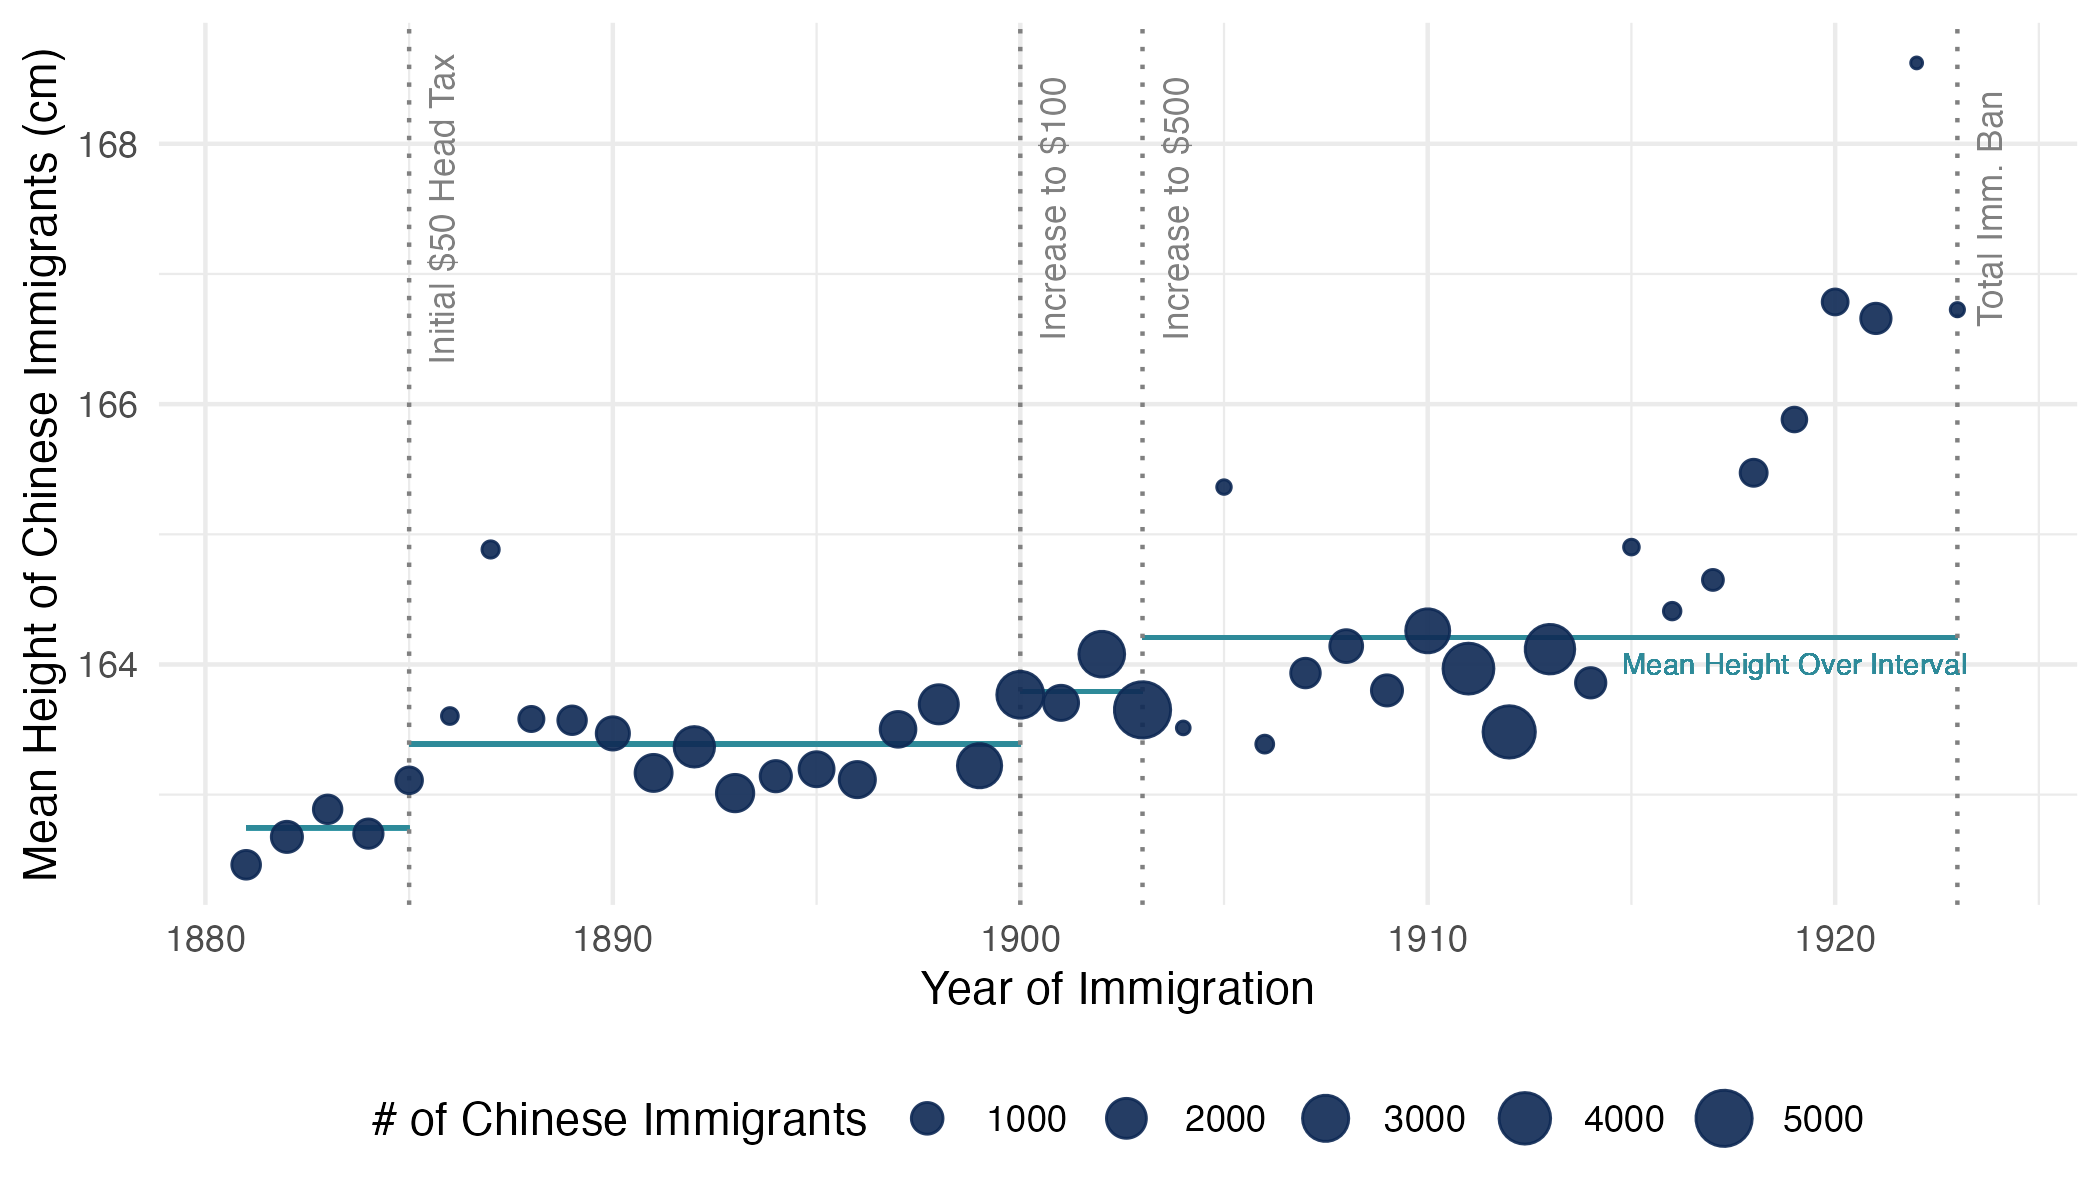
\includegraphics[width=\textwidth]{../../figs/height_selection.png}
    \label{fig:height_selection}
\end{figure}

\noindent \textbf{Evolution of Selection} \par 
Figure \ref{fig:height_selection} graphs the average height of Chinese immigrant men between ages 23 and 50 by year of arrival in Canada, with larger points representing years with more Chinese immigrants. As discussed above, the average height of Chinese immigrant men under the \$50 Head Tax was 163.4cm, which corresponds to neutral or slightly positive selection on height relative to the Chinese population. The average height of Chinese immigrants, however, rises to 163.8cm under the \$100 Head tax and 164.2cm under the \$500 Head Tax, indicating that the selection of Chinese immigrants to Canada on height became increasingly positive as the cost of migration increased.\footnote{The rapid increase in the average height of Chinese immigrants to nearly 167cm by the 1920s was driven by a small number of non-taxpayers, who were mostly students.}

The literature on historical Chinese height indicates that accounting for birth cohort effects suggests an even larger increase in selection, since a wide range of other data sources consistently show a 1-2cm decrease in the average height of Chinese men between the 1850 birth cohort and the 1890 birth cohort \citep{batenetal2010}. These roughly correspond to the immigrant cohorts of 1880 and 1920 respectively, indicating that all else equal, average heights would have decreased over this time period. Instead, average heights increased, indicating that selection into immigration from China to Canada became increasingly positive as the Head Tax grew. This is again in line with the predictions of the \citet{chiquiarhanson2005} selection model. 

%In the following sections, I formally test whether selection becomes more positive (i.e. the average skill of immigrants increases) as the Head Tax grows.

% While it is difficult to directly estimate the returns to skill in China relative to Canada in the 19th and early 20th centuries due to a dearth of Chinese income or education data, I can use several results from the historical literature to draw conclusions about the nature of selection of Chinese immigrants to Canada in the late 1800's.

% First, I observe that 96\% of Chinese immigrants to Canada are listed as originating from Guangdong province, a region of Southern China that borders Hong Kong and Macau, and served as the primary trade port between China and the Western world.

% First, existing approximations of the distribution of income in China and Canada in 1880 by \citet{chancelpiketty2021} do not yield 


\subsection{Empirical Specification}
While the above analysis is indicative of selection into immigration relative to the Chinese population becoming more positive as the Head Tax increased, the drawback of using Register data to measure selection of Chinese immigrants is that there is no counterfactual group of immigrants against which to measure changes in the Chinese immigrant pool due to the Head Tax. Therefore we can not rule out that all immigrants to Canada are also becoming more positively selected over this time period due to factors unrelated to the Head Tax. Using Canadian census data, I am able to compare the characteristics of Chinese and non-Chinese immigrants over time, accounting for any Canada-specific `pull' factors that might have affected the selection of all immigrant groups over time. 

My main empirical strategy to compare changes in the composition of Chinese and non-Chinese immigrants uses the standard difference-in-differences design. My preferred specification is as follows:

\begin{equation}
    \label{eq:did}
    y_{ict} = \beta_1 BORNCHI_i + \beta_2 AGE_{ic} + \delta_c + \delta_t + \sum_{\tau \in \mathcal{T}^d} \gamma_\tau^{DD} \times BORNCHI_i \times \mathbf{1}[TAX_t = \tau] + \varepsilon_{ict}
\end{equation}

where $i$ indexes individuals, $c$ indexes census year, and $t$ indexes year of immigration. 
$BORNCHI_i$ is an indicator for whether an individual was born in China (a proxy for being a Chinese immigrant), $AGE_{ic}$ represents the age of individual $i$ in census year $c$, $TAX_t$ represents the head tax amount in year $t$, and $y_{ict}$ is the characteristic or outcome of interest. $\beta_1$ captures the baseline effect of being a Chinese immigrant, $\beta_2$ captures a linear age effect, $\delta_c$ caputres census year fixed effects, and $\delta_t$ captures year fixed effects. My main object of interest is $\gamma_{\tau}^{DD}$ which captures the effect of having immigrated in a year with Head Tax $\tau$ \textbf{and} being Chinese.

The estimating equation is identified under the assumption that without the Head Tax, the characteristics of Chinese and non-Chinese immigrants would have evolved similarly. If this assumption is met, $\gamma_{\tau}^{DD}$ represents the effect of a Head Tax of $\tau$ on some measure of selection of the immigrant population.\footnote{For example, if $y$ is an indicator for literacy, $\gamma_{500}^{DD}$ represents the difference between the actual literacy rate of the Chinese immigrants that immigrated under the \$500 Head Tax and the counterfactual literacy rate of the Chinese immigrants that would have immigrated over the same time period if the Head Tax had not been in place.} This serves as a proxy for the effect of an increase in migration costs on selection, under the additional assumption that other migration costs evolved similarly for Chinese and non-Chinese migrants over this time period.

It is reasonable to assume that immigration pattern for Chinese and non-Chinese immigrants would have changed similarly over this time period in the absence of the Head Tax. No single immigrant group between 1880 and 1913 was large enough for idiosyncratic country `push' factors to have a large impact on the overall composition of immigrants, and this time period excludes worldwide events that would have affected immigration across many countries, such as World War I. Nevertheless, although there were no major historical events that would have affected Chinese immigration specifically during this time period,\footnote{Events such as the Opium Wars and the Taiping rebellion spurred waves of Chinese immigration in the mid-1800s \citep{mckeown2010}.} it is possible that internal economic factors may have caused Chinese immigration to evolve differently from other countries. 

To this end, I supplement my analysis with an alternative sample containing only Chinese and Japanese immigrants, effectively using only Japanese immigrants as the comparison group, following work by \citet{Chen2015}. Not only were there economic and cultural similarities between Japanese and Chinese immigrants at the time, the actual voyage to Canada was typically on the same boat, which would make stops in both Hong Kong and Yokohama, increasing the likelihood that migration costs of Japanese and Chinese immigrants would have been directly comparable without the Head Tax.

\subsection{Results}

\begin{table}[!h]
    \centering 
    \renewcommand{\arraystretch}{1.3}
    \resizebox{\textwidth}{!}{
    \begin{threeparttable}
        \caption{Regression results from Equation (\eqref{eq:did}) showing the relationship between the Chinese Head Tax and the composition of Chinese immigrants, as compared to all immigrants in columns (1)-(3) and Japanese immigrants only in columns (4)-(6), using pooled Canadian census data from 1901, 1910, and 1921 \citep{census1901,census1911,census1921}.}
        \label{tab:selection}
        
% Table created by stargazer v.5.2.3 by Marek Hlavac, Social Policy Institute. E-mail: marek.hlavac at gmail.com
% Date and time: Fri, Oct 20, 2023 - 18:56:40
\begin{tabular}{@{\extracolsep{5pt}}lcccccc} 
\\[-1.8ex]\hline 
\hline \\[-1.8ex] 
 & \multicolumn{3}{c}{All Immigrants (1880-1913)} & \multicolumn{3}{c}{Chinese \& Japanese Imm. (1890-1907)} \\ 
 & \multicolumn{6}{c}{\textit{Dependent variable:}} \\ 
\cline{2-7} 
\\[-1.8ex] & $\mathbb{P}[\text{Laborer}]$ & $\mathbb{P}[\text{Literate}]$ & $\mathbb{P}[\text{Owns House}]$ & $\mathbb{P}[\text{Laborer}]$ & $\mathbb{P}[\text{Literate}]$ & $\mathbb{P}[\text{Owns House}]$ \\ 
\\[-1.8ex] & (1) & (2) & (3) & (4) & (5) & (6)\\ 
\hline \\[-1.8ex] 
 $\hat{\beta}_{1}$ ($BORNCHI$) & 0.252$^{***}$ & $-$0.396$^{***}$ & $-$0.497$^{***}$ & 0.056$^{*}$ & 0.023 & $-$0.131$^{***}$ \\ 
  & (0.032) & (0.024) & (0.038) & (0.031) & (0.035) & (0.025) \\ 
  & & & & & & \\ 
 $\hat{\gamma}_{50}^{DD}$ ($BORNCHI \times$ \$50 Tax) & $-$0.038 & 0.181$^{***}$ & 0.101$^{**}$ &  &  &  \\ 
  & (0.035) & (0.027) & (0.041) &  &  &  \\ 
  & & & & & & \\ 
 $\hat{\gamma}_{100}^{DD}$ ($BORNCHI \times$ \$100 Tax) & 0.035 & 0.200$^{***}$ & 0.014 & 0.050 & 0.080 & $-$0.007 \\ 
  & (0.039) & (0.029) & (0.046) & (0.075) & (0.079) & (0.060) \\ 
  & & & & & & \\ 
 $\hat{\gamma}_{500}^{DD}$ ($BORNCHI \times$ \$500 Tax) & $-$0.132$^{***}$ & 0.120$^{***}$ & 0.133$^{***}$ & $-$0.117$^{**}$ & $-$0.114$^{**}$ & 0.014 \\ 
  & (0.034) & (0.026) & (0.040) & (0.052) & (0.055) & (0.042) \\ 
  & & & & & & \\ 
Dep. Var. Mean (SE) & 0.2081 & 0.9167 & 0.5146 & 0.3559 & 0.6878 & 0.1877 \\ 
 & (0.0017) & (0.0012) & (0.0022) & (0.0106) & (0.0112) & (0.0087) \\ 
\hline \\[-1.8ex] 
Observations & 55,149 & 56,156 & 57,148 & 2,190 & 1,864 & 2,190 \\ 
Adjusted R$^{2}$ & 0.062 & 0.050 & 0.123 & 0.017 & 0.008 & 0.060 \\ 
\hline \\[-1.8ex] 
\end{tabular} 

        \begin{tablenotes}
            \item $^{*}$p$<$0.1; $^{**}$p$<$0.05; $^{***}$p$<$0.01
            \item 
            \item \textbf{Notes:} $\mathbb{P}[\text{Laborer}]$ is an indicator for having the occupation ``Labourer'', including farm labor, $\mathbb{P}[\text{Literate}]$ is an indicator for being literate in any language, as recorded by the census enumerator, and $\mathbb{P}[\text{Own House}]$ is an indicator for owning property, including one's own house. 
            The sample, using 1901-1921 Canadian Census data \citep{census1901, census1911,census1921}, is restricted to men who were 18 or older at the time of arrival, to reduce the effect of differential assimilation of children of different immigrant groups. As specified in Section 2.2, I restrict the ``All Immigrants'' sample to arrivals prior to 1914 due to the potential effects of World War I, and I restrict the Japanese sample to arrivals prior to 1908 due to restrictions on Japanese immigration that began in 1908. Additionally, because very few Chinese immigrants arrived prior to 1880 and very few Japanese immigrants arrived prior to 1890, I restrict the ``All Immigrants'' sample to arrivals after 1880 and I restrict the Japanese sample to arrivals after 1890. 
        \end{tablenotes}
    \end{threeparttable}
    }
\end{table}


I use three measures of selection from the Canadian census: an indicator for working as a laborer, an indicator for literacy, and an indicator for property ownership. I report the results of estimating equation \eqref{eq:did} with each of these outcome variables in Table \ref{tab:selection}.

Columns (1)-(3) use all non-Chinese immigrants as a control group, and my estimates of $\gamma_{500}^{DD}$ indicate that Chinese immigrants who arrived under the largest (\$500) Head Tax, were less likely to be laborers, more likely to be able to read, and more likely to own property, relative to immigrants in years with no Head Tax, all of which suggest relatively more positive selection. Comparing the \$50 Head Tax to no Head Tax also suggests significantly more positive selection, but results for LABOR and HOUSEOWN under the \$100 Head Tax are insignificant -- likely because the \$100 Head Tax only spanned three years, 1901-1903.
%\footnote{Note that in addition, these years were immediately following the 1901 census, and so would have been heavily affected by outmigration relative to other periods. In other words, only immigrants who arrived within that three year span and stayed in Canada for at least eight years (until the next census in 1911) would have been counted as having arrived under the \$100 Head Tax.}

As noted in Section 6.2, however, these results rely on the assumption that in the absence of the Head Tax, the characteristics of Chinese immigrants and the characteristics of all other immigrants would have evolved similarly, which may not have been the case, even with the exclusion of World War I and following years. I repeat estimation of equation (\eqref{eq:did}) using only Japanese immigrants as the comparison group, who (as noted above) were much more likely to have evolved similarly to Chinese immigrants over this time period in the absence of the Head Tax. Due to the fact that Japanese immigration to Canada was largely nonexistent prior to 1890 (only 26 Japanese immigrants in the pooled 1901-1921 Canadian Census sample arrived prior to 1890), I restrict the sample to immigrants who arrived beginning in 1890, so I am required to use the \$50 Head tax as the omitted group. Nevertheless, I still find estimates that are largely consistent with columns (1)-(3).
Relative to those who immigrated under the \$50 Head Tax, Chinese immigrants who immigrated under the \$500 Head Tax were significantly less likely to be working as laborers, and more likely to own property (although this result is indistinguishable from zero). 

An interesting result from both the Japanese sample in column (5) and the All Immigrants sample in column (2) is that Chinese immigrants under the \$500 Head Tax were actually less likely to be literate than Chinese immigrants under the \$50 Head Tax, compared to Japanese immigrants and compared to all immigrants. This may be due to underlying differences in how literacy evolved in China relative to other countries over this time period, or it may suggest that the increasingly positive selection of Chinese immigrants over this period was independent of or even negatively correlated with literacy. 
For instance, if literacy for Chinese men was positively correlated with wages in China but not in Canada, and if height was independent of literacy, then positive selection on the basis of height would generate negative selection on the basis of literacy, since the highly literate would have no height advantage and higher returns to literacy in China.\footnote{This is related to work by \citet{gouldmoav2016} on country-specific and general skills in the context of Israeli emigrants.}


In summary, my results are broadly consistent with migration cost inducing more positive selection into immigration, particularly based on wealth and occupation. 


% Age heaping is a measure of numeracy based on the tendency of the less educated to report ages in multiples of 5 \citep{mokyrgrada1982,humphriesleunig2009,stolzbaten2012} -- I define $AGEHEAP_{ict} = \mathbbm{1}[\text{Reported age ends in 0 or 5}]$. 

% \begin{table}[!h]
%     \centering 
%     \renewcommand{\arraystretch}{1.5}
%     \resizebox{\textwidth}{!}{
%     \begin{threeparttable}
%         \caption{Regression results from Equation \eqref{eq:did} showing the relationship between the Chinese Head Tax and Chinese immigrant outcomes in Canada.}
%         \label{tab:outcomes_match}
%         
% Table created by stargazer v.5.2.3 by Marek Hlavac, Social Policy Institute. E-mail: marek.hlavac at gmail.com
% Date and time: Wed, Apr 12, 2023 - 13:23:13
\begin{tabular}{@{\extracolsep{5pt}}lcccccccc} 
\\[-1.8ex]\hline 
\hline \\[-1.8ex] 
 & \multicolumn{4}{c}{Sample: All Immigrants} & \multicolumn{4}{c}{Sample: Chinese and Matched Immigrants} \\ 
 & \multicolumn{8}{c}{\textit{Dependent variable:}} \\ 
\cline{2-9} 
\\[-1.8ex] & $LABORER$ & $LITERATE$ & $EARNINGS$ & $HOMEOWN$ & $LABORER$ & $LITERATE$ & $EARNINGS$ & $HOMEOWN$ \\ 
\\[-1.8ex] & (1) & (2) & (3) & (4) & (5) & (6) & (7) & (8)\\ 
\hline \\[-1.8ex] 
 $BORNCHI$ & 0.170$^{***}$ & $-$0.309$^{***}$ & $-$240.600$^{***}$ & $-$0.271$^{***}$ & 0.297$^{***}$ & $-$0.391$^{***}$ & $-$116.700$^{***}$ & $-$0.217$^{***}$ \\ 
  & (0.023) & (0.019) & (39.590) & (0.025) & (0.038) & (0.032) & (40.600) & (0.043) \\ 
  & & & & & & & & \\ 
 $BORNCHI \times$ \$100 Tax & $-$0.056 & 0.121$^{***}$ & 158.000$^{**}$ & $-$0.064 & $-$0.062 & 0.042 & 255.100$^{**}$ & 0.340$^{***}$ \\ 
  & (0.040) & (0.029) & (65.280) & (0.044) & (0.109) & (0.093) & (114.700) & (0.125) \\ 
  & & & & & & & & \\ 
 $BORNCHI \times$ \$500 Tax & $-$0.066$^{**}$ & 0.043$^{**}$ & 24.890 & $-$0.052$^{*}$ & $-$0.239$^{***}$ & 0.054 & $-$64.050 & $-$0.055 \\ 
  & (0.026) & (0.020) & (43.770) & (0.029) & (0.046) & (0.037) & (46.560) & (0.053) \\ 
  & & & & & & & & \\ 
Includes Year FE & Yes & Yes & Yes & Yes & Yes & Yes & Yes & Yes \\ 
\hline \\[-1.8ex] 
Observations & 42,058 & 41,212 & 40,409 & 42,058 & 2,022 & 1,747 & 1,904 & 2,022 \\ 
Adjusted R$^{2}$ & 0.025 & 0.042 & 0.067 & 0.078 & 0.259 & 0.281 & 0.359 & 0.244 \\ 
\hline \\[-1.8ex] 
\end{tabular} 

%         \begin{tablenotes}
%             \item $^{*}$p$<$0.1; $^{**}$p$<$0.05; $^{***}$p$<$0.01
%             \item 
%             \item \textbf{Notes:} Analysis in this table uses only Canadian census data from 1901-1921. As in Table \ref{tab:immflow}, immigrants are only counted in the closest subsequent census from their year of arrival. Unlike in Table \ref{tab:immflow}, I further restrict the sample such that only immigrants who arrived after 1890 and prior to 1921 are included, which ensures that there is a maximum of 10 years between arrival and being recorded in the census (allowing for uniformity across census years of attrition bias due to outmigration). Columns (1)-(4) use all immigrants to Canada during this time period, while columns (5)-(8) restrict the sample to only Chinese and matched immigrants.
%         \end{tablenotes}
%     \end{threeparttable}
%     }
% \end{table}

% I now turn to focus on the relationship between the head tax and outcomes for Chinese immigrants after arrival, estimated using the following equation: 
% \begin{equation}
%     \label{eq:did}
%     y_{it} = \delta_t + \alpha BORNCHI_i + \sum_{k \in \{100, 500\}} \gamma_k BORNCHI_i \times \mathbf{1}[TAX_t = k] + \varepsilon_{it}
% \end{equation}

% where $i$ indexes individuals, $t$ indexes year of immigration, $BORNCHI_i$ is an indicator for whether an individual was born in China (a proxy for being a Chinese immigrant), $TAX_t$ represents the head tax amount in year $t$, and $y_{it}$ is the outcome of interest. $\alpha$ captures the baseline effect of being a Chinese immigrant, $\delta_t$ captures year fixed effects, and $\gamma_k$ captures the effect of the \$100 and \$500 head tax, with the \$50 head tax as the omitted category.\footnote{I restrict the sample to immigrants who arrived between 1891 and 1921, thus omitting any Chinese immigrants who would have paid \$0 in taxes at the time of entry. This is because there were relatively very few Chinese immigrants who immigrated before 1885 (and paid no tax at the time of entry), especially as reported in the 1901-1921 censuses (the years which include Year of Immigration as a variable).} 
% Note that only one census (the closest census year $c$ such that $c > t$) is used to measure each year of immigration $t$, so $\delta_t$ also captures effects of the census year and the effects of the number of years since immigration. 

% The results of estimating Equation \eqref{eq:did} for outcome variables $LABORER$ (an indicator for if person $i$'s primary occupation is laborer), $LITERATE$ (an indicator for whether person $i$ is literate), $EARNINGS$ (annual earnings), and $HOMEOWN$ (an indicator for whether person $i$ owns their own home) are displayed in Table \ref{tab:outcomes}. Columns (1)-(4) use all adult male immigrants as the sample (effectively comparing Chinese immigrants to all other immigrants), while columns (5)-(8) use only Chinese and Japanese adult male immigrants as the sample (only comparing Chinese immigrants to Japanese immigrants). 
% As described in Table \ref{tab:summstats}, and as verified in the first row of columns (1)-(4), Chinese immigrants to Canada are more likely to be a laborer and less likely to be literate than other immigrants. Additionally, they make less in annual earnings and are less likely to own their own home than other immigrants. The first row of columns (5)-(8) show, however, that Chinese immigrants are much more comparable with Japanese immigrants. In the period sampled, Chinese and Japanese immigrants to Canada are not statistically significantly different in their likelihood of being a laborer, in their annual earnings, or in their probability of owning a home, although Chinese immigrants are still less likely to be literate than Japanese immigrants. This suggests that narrowing the sample to only Chinese and Japanese immigrants may help control for conditions in Canada after arrival, as well as other underlying differences in the immigrant population.

% Column (1) shows that immigrating from China in a year with a higher head tax is associated with a lower likelihood of being a laborer, relative to all other immigrants. In particular, an immigrant from China who pays a \$500 head tax is 6.6 percentage points less likely to be a laborer than an immigrant from China who pays a \$50 head tax. This is suggestive of some selection effect of the head tax -- higher head taxes attract immigrants who are more skilled and can work in non-laborer positions. Another possibility, however, is that there were just fewer laborer jobs available to Chinese immigrants in the years when the head tax was higher. 
% Column (5) provides evidence against this latter explanation -- even when comparing Chinese immigrants with only Japanese immigrants, who presumably faced similar job markets, being a Chinese immigrant in a year with a higher head tax is associated with a lower probability of being a laborer, although the magnitude of the effect is smaller.

% Columns (2) and (6) further support the theory that higher head taxes induced more positive selection into immigration, showing that Chinese immigrants who faced higher head taxes were more likely to be able to read English, although the effect is unexpectedly stronger for the \$100 tax than for the \$500 tax. Column (3) shows a similar pattern, where Chinese immigrants who paid the \$100 head tax are likely to be earning more than those who paid the \$50 head tax, although the effect is again smaller for immigrants who paid the \$500 head tax. Once Chinese immigrants are compared with a more similar group, however, in column (7), this positive selection effect disappears and there is actually a negative effect on earnings. This suggests that whatever selection effect contributes to a lower likelihood of being a laborer is dominated by negative effect on wages. 
% One possibility is that a higher head tax reduced new immigrants' savings, potentially even inducing some immigrants to borrow and causing immigrants to be willing to accept lower wages, despite higher skills.

% Columns (4) and (8) support this theory, showing that there is also a significantly negative effect on home ownership. A negative effect on home ownership is a strong signal of a negative effect on wealth (especially when compared with Japanese immigrants who likely faced similar housing markets and discrimination), and this suggests that Chinese immigrants facing higher head taxes did in fact experience significant setbacks that made it harder for them to accumulate wealth and purchase homes.

% \subsection{Comparing Canada to the US}

% \begin{figure}
%     \centering 
%     \caption{Inflow of Chinese immigrants to Canada and the US, as measured by the Canadian and US Censuses.}
%     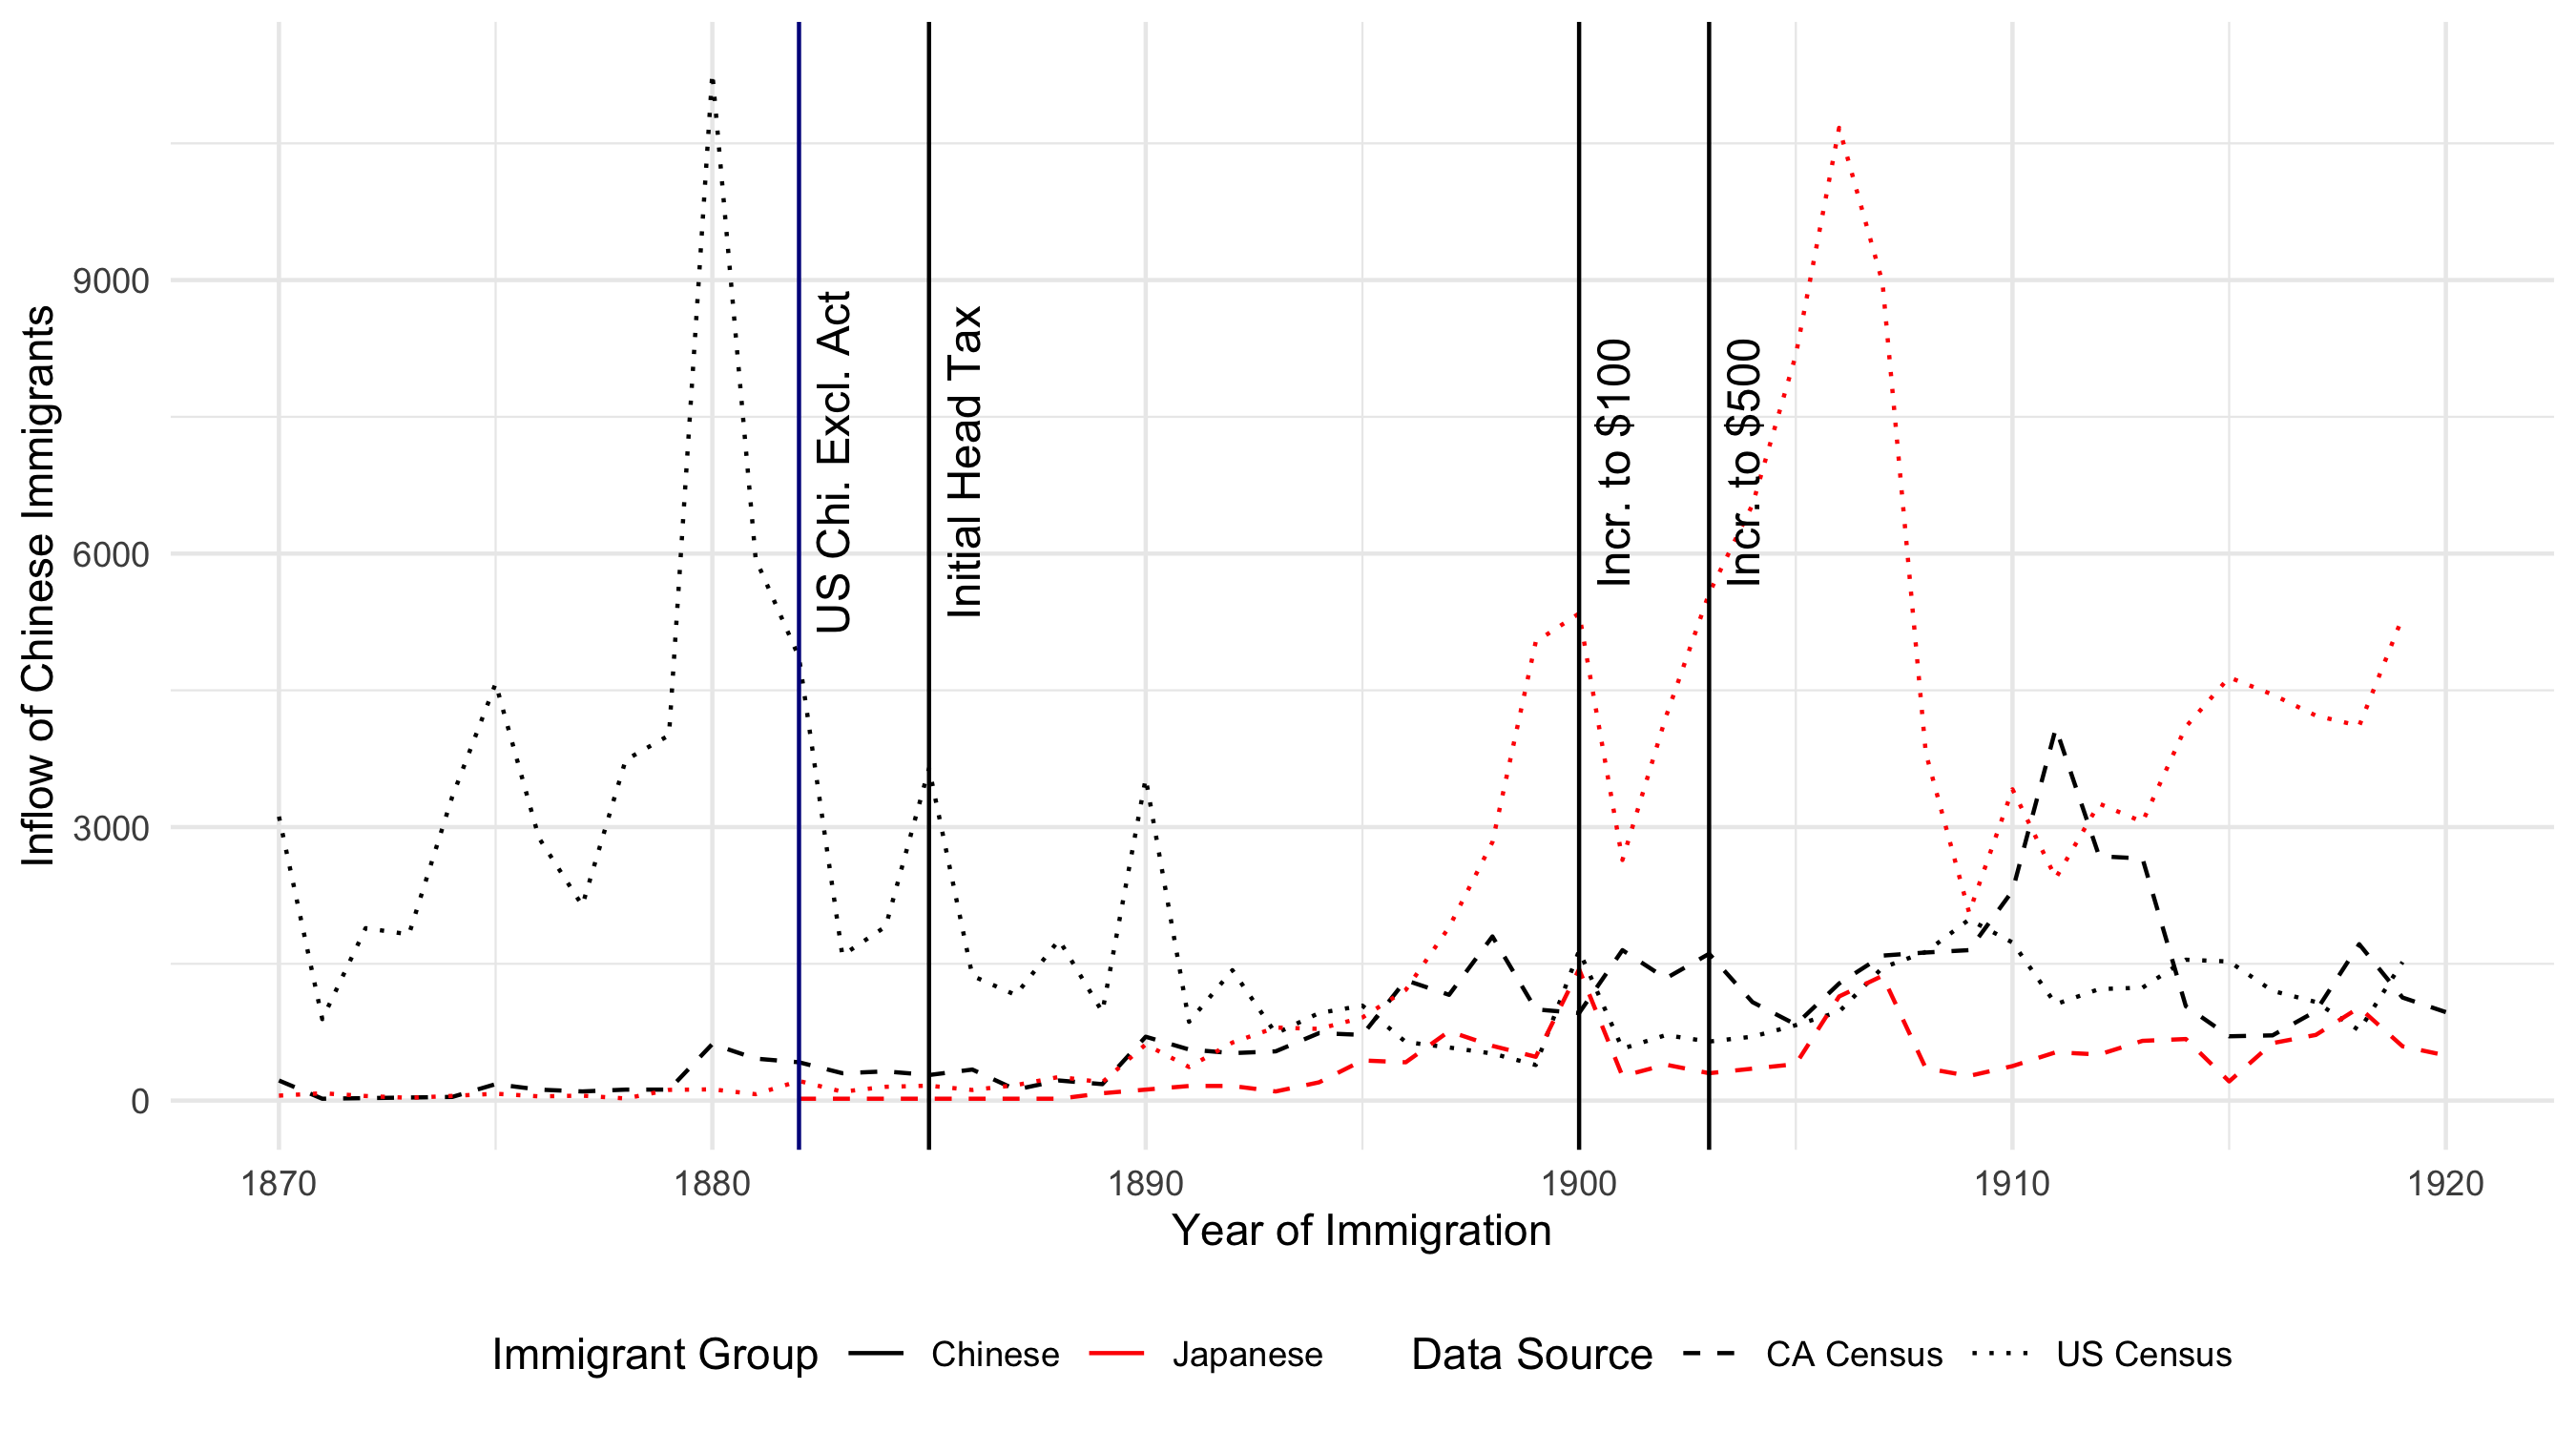
\includegraphics[width=\textwidth]{../../figs/fig3_us_can.png}
%     \label{fig:taxpaid}
% \end{figure}

% The above analysis relies on the assumption above that in the absence of the head tax, the outcomes of Japanese and Chinese immigrants to Canada would have evolved similarly. In reality, it is likely that there were China-specific immigration shifters that would have affected Chinese immigration to Canada differently over time. In this section, I control for supply-side shocks by estimating the following equation:

% \begin{multline}
%     \label{eq:uscan}
%     y_{ict} = \delta_{ct} + \sum_{c \in \{US, \, Canada\}} \alpha_c BORNCHI_i \times \mathbf{1}[COUNTRY_i = c] \\ + \sum_{k \in \{100,500\}, \, c \in \{US, \, Canada\}} \gamma_{ck} BORNCHI_i \times \mathbf{1}[COUNTRY_i = c] \times \mathbf{1}[TAX_t = k] + \varepsilon_{ict}
% \end{multline}

% where $c \in \{US, \, Canada\}$ indexes country, the coefficients $\alpha_c$ and $\gamma_{ck}$ now vary by country of arrival, and $\delta_{ct}$ now represents Year $\times$ Country fixed effects. 

% \begin{table}[!h]
%     \centering 
%     \renewcommand{\arraystretch}{1.1}
%     \resizebox{0.7\textwidth}{!}{
%     \begin{threeparttable}
%         \caption{Regression results from Equation \eqref{eq:uscan} showing the relationship between the Chinese Head Tax and Chinese immigrant outcomes in Canada as compared to the US.}
%         \label{tab:uscanregs}
%         
% Table created by stargazer v.5.2.3 by Marek Hlavac, Social Policy Institute. E-mail: marek.hlavac at gmail.com
% Date and time: Sat, Apr 01, 2023 - 00:36:30
\begin{tabular}{@{\extracolsep{5pt}}lccc} 
\\[-1.8ex]\hline 
\hline \\[-1.8ex] 
 & \multicolumn{3}{c}{Sample: Chinese and Japanese Immigrants} \\ 
\cline{2-4} 
\\[-1.8ex] & LABORER & LITERATE & HOMEOWN \\ 
\\[-1.8ex] & (1) & (2) & (3)\\ 
\hline \\[-1.8ex] 
$BORNCHI \times US$ & $-$0.228$^{***}$ & $-$0.109$^{***}$ & $-$0.027$^{***}$ \\ 
& (0.009) & (0.007) & (0.006) \\ 
& & & \\ 
$BORNCHI \times CANADA $ & 0.252$^{***}$ & $-$0.057$^{***}$ & 0.041$^{***}$ \\ 
& (0.014) & (0.014) & (0.010) \\ 
& & & \\ 
$BORNCHI \times US \times $ \$100 Tax & 0.087$^{***}$ & 0.026$^{**}$ & $-$0.006 \\ 
& (0.014) & (0.012) & (0.010) \\ 
& & & \\ 
$BORNCHI \times US \times $ \$500 Tax & 0.062$^{***}$ & 0.048$^{***}$ & 0.012$^{*}$ \\ 
& (0.010) & (0.008) & (0.007) \\ 
& & & \\ 
$BORNCHI \times CANADA \times $ \$100 Tax & $-$0.256$^{***}$ & 0.298$^{***}$ & $-$0.114$^{***}$ \\ 
& (0.025) & (0.024) & (0.017) \\ 
& & & \\ 
$BORNCHI \times CANADA \times $ \$500 Tax & $-$0.112$^{***}$ & 0.010 & $-$0.118$^{***}$ \\ 
& (0.017) & (0.016) & (0.012) \\ 
& & & \\ 
Includes Year $\times$ Country FE & Yes & Yes & Yes \\ 
\hline \\[-1.8ex] 
Observations & 109,012 & 108,639 & 109,012 \\ 
Adjusted R$^{2}$ & 0.061 & 0.079 & 0.032 \\ 
\hline \\[-1.8ex] 
\end{tabular} 

%         \begin{tablenotes}
%             \item $^{*}$p$<$0.1; $^{**}$p$<$0.05; $^{***}$p$<$0.01
%             \item 
%             \item \textbf{Notes:} Analysis in this table uses Canadian census data from 1901-1921 and US census data from 1900-1920. As in Table \ref{tab:outcomes} I restrict the sample such that only immigrants who arrived after 1890 and prior to 1920 are included (since the latest US census year I use is 1920). All columns restrict the sample to only Chinese and Japanese immigrants from the US and Canada.
%         \end{tablenotes}
%     \end{threeparttable}
%     }
% \end{table}

% Results of estimating Equation \eqref{eq:uscan} for the sample of Chinese and Japanese immigrants to Canada who arrived between 1890 and 1920 are presented in Table \ref{tab:uscanregs}. Observe that Canadian Chinese immigrants are significantly less literate and more likely to be laborers than US Chinese immigrants, as suggested by summary statistics in Table \ref{tab:summstats}, and are also less likely to own their own home. Lines 3 and 4 represent the impact of Chinese immigrants to the US arriving in years with a higher \textbf{Canadian} head tax, which I would expect to be minimal, but I in fact observe to be significant. This suggests that the head tax may have had some spillover effects on Chinese immigration to the US. 

% Column (1) shows that while Chinese immigrants to Canada in higher head tax years are less likely to be laborers (in line with the selection effect observed above), Chinese immigrants to the US in higher head tax years are in fact \textbf{more} likely to be laborers. This actually lends support to the selection theory, since the lower-skilled immigrants who could not afford the higher head tax may have substituted towards immigration to the US (although the existence of the Chinese Exclusion Act during this time period, which prohibited immigration of laborers, complicates this theory). 

% Column (2) shows that immigrating in years with higher head taxes is associated with higher literacy rates for Chinese immigrants to both the US and Canada -- this is a puzzling result, as it does not accord with a theory of substitution between the US and Canada. Earnings are not included as an outcome variable because they are not available in the US census data during this time period, however column (3) presents results for home ownership. The results are again in line with my findings in Table \ref{tab:outcomes}, and the very small and mostly insignificant effects for Chinese immigrants to the US further suggests that the wealth effect (which does not affect Chinese immigrant outcomes in the US) dominates the selection effect (which would potentially spillover to Chinese immigrant outcomes in the US) for the outcome of home ownership.